\documentclass[11pt]{article}
\usepackage{wasysym}
\usepackage{listings}
\usepackage{tikz}
\usepackage{url}
%\usepackage{algorithm2e}
\usetikzlibrary{arrows,automata,shapes}
\tikzstyle{block} = [rectangle, draw, fill=blue!20, 
    text width=2.5em, text centered, rounded corners, minimum height=2em]
\tikzstyle{bw} = [rectangle, draw, fill=blue!20, 
    text width=3.5em, text centered, rounded corners, minimum height=2em]

\newcommand{\handout}[5]{
  \noindent
  \begin{center}
  \framebox{
    \vbox{
      \hbox to 5.78in { {\bf ECE459: Programming for Performance } \hfill #2 }
      \vspace{4mm}
      \hbox to 5.78in { {\Large \hfill #5  \hfill} }
      \vspace{2mm}
      \hbox to 5.78in { {\em #3 \hfill #4} }
    }
  }
  \end{center}
  \vspace*{4mm}
}

\newcommand{\lecture}[4]{\handout{#1}{#2}{#3}{#4}{Lecture #1}}
\topmargin 0pt
\advance \topmargin by -\headheight
\advance \topmargin by -\headsep
\textheight 8.9in
\oddsidemargin 0pt
\evensidemargin \oddsidemargin
\marginparwidth 0.5in
\textwidth 6.5in

\parindent 0in
\parskip 1.5ex
%\renewcommand{\baselinestretch}{1.25}

\begin{document}
\lecture{3 --- January 9, 2015}{Winter 2015}{Patrick Lam}{version 1}


\paragraph{Generalizing Amdahl's Law.} We made a simplification,
which was that programs only have one parallel part and one serial part.
Of course, this is not true. The program may have many parts,
each of which we can tune to a different degree.

Let's generalize Amdahl's Law:

\begin{itemize}
\item  $f_1, f_2, \ldots, f_n$: fraction of time in part $n$
\item  $S_{f_1}, S_{f_n}, \ldots, S_{f_n}$: speedup for part $n$
\end{itemize}

Then,
\[\mbox{\em speedup} = \frac{1}{\frac{f_1}{S_{f_1}} + \frac{f_2}{S_{f_2}} + \ldots +
    \frac{f_n}{S_{f_n}}}.\]

\paragraph{Example.} Consider a program with 4 parts in the following scenario:

\begin{center}
    \begin{tabular}{r|r|r|r}
    \multicolumn{2}{l}{} & \multicolumn{2}{|c}{Speedup} \\
    Part & Fraction of Runtime & Option 1 & Option 2\\
    \hline
    1 & 0.55 & 1  & 2\\
    2 & 0.25 & 5  & 1\\
    3 & 0.15 & 3  & 1\\
    4 & 0.05  & 10 & 1\\
    \end{tabular}
\end{center}

    (Note: these speedups don't have to be speedups from parallelization.)
    
  We can implement either Option 1 or Option 2. 
  Which option is better?

  ``Plug and chug'' the numbers:
\begin{itemize}
\item  {\bf Option 1.}

  \[ \mbox{\em speedup} = \frac{1}{0.55 + \frac{0.25}{5} + \frac{0.15}{3} + \frac{0.05}{5}}
    = 1.53  \]

\item  {\bf Option 2.}

  \[\mbox{\em speedup} = \frac{1}{\frac{0.55}{2} + 0.45} = 1.38 \hspace*{5.5em}\]
\end{itemize}

   \paragraph{Empirically estimating parallel speedup $P$.}
Assuming that you know things that are actually really hard to know, here's a formula for estimating speedup. You don't have to commit it to memory:
  \[P_{\mbox{\scriptsize estimated}} = \frac{\frac{1}{\mbox{\em speedup}}-1}{\frac{1}{N}-1}.\]

It's just an estimation, but you can use it to guess the fraction of parallel code, given $N$ and the speedup. You can then use $P_{\mbox{\scriptsize estimated}}$ to predict speedup for a different number of processors.

\subsection*{A more optimistic point of view}
In 1988, John Gustafson pointed
out\footnote{\url{http://www.scl.ameslab.gov/Publications/Gus/AmdahlsLaw/Amdahls.html}}
that Amdahl's Law only applies to fixed-size problems, but that the
point of computers is to deal with bigger and bigger problems.

In particular, you might vary the input size, or the grid resolution,
number of timesteps, etc. When running the software, then, you might
need to hold the running time constant, not the problem size: you're
willing to wait, say, 10 hours for your task to finish, but not 500
hours. So you can change the question to: how big a problem can you
run in 10 hours?

According to Gustafson, scaling up the problem tends to increase the
amount of work in the parallel part of the code, while leaving the
serial part alone. As long as the algorithm is linear, it is possible
to handle linearly larger problems with a linearly larger number of
processors.

Of course, Gustafson's Law works when there is some ``problem-size''
knob you can crank up.  As a practical example, observe Google, which
deals with huge datasets.

\section*{Concurrency and Parallelism}
Concurrency and parallelism both give up the
total ordering between instructions in a sequential program, for
different purposes.

\paragraph{Concurrency.} We'll refer to the use of threads for
structuring programs as concurrency. Here, we're not aiming
for increased performance. Instead, we're trying to write the program
in a natural way. Concurrency makes sense as a model for distributed
systems, or systems where multiple components interact, with no ordering
between these components, like graphical user interfaces.

\paragraph{Parallelism.} We're studying parallelism in this class, where
we try to do multiple things at the same time in an attempt to increase
throughput. Concurrent programs may be easier to parallelize.

\newpage
\section*{Processor Design Issues}
Recall that we listened to Cliff Click describe characteristics of
modern processors in Lecture 2. In this lecture we'll continue our
quick review of computer architecture and how it relates to
programming for performance. Here's another reference about chip
multi-threading; we are going to study some
of the techniques in the ``Writing Scalable Low-Level Code'' section.

\begin{center}
\url{http://queue.acm.org/detail.cfm?id=1095419}
\end{center}

\paragraph{Processes and Threads.} Let's review the
difference between a process and a thread. A \emph{process} is an
instance of a computer program that contains program code and its own
address space, stack, registers, and resources (file handles, etc).  A
\emph{thread} usually belongs to a process. The most important point
is that it shares an address space with its parent process, hence
variables and code as well as resources. Threads have their own stack,
registers, and thread-specific data.

\paragraph{Threads and CPUs.} In your operating systems class,
you've seen implementations of threads (``lightweight processes'').
We'll call these threads \emph{software threads}, and we'll program
with them throughout the class. Each software thread corresponds to a
stream of instructions that the processor executes. On a old-school
single-core, single-processor machine, the operating system
multiplexes the CPU resources to execute multiple threads
concurrently; however, only one thread runs at a time on the single
CPU.

On the other hand, a modern chip contains a number of \emph{hardware
threads}, which correspond to the virtual CPUs. These are sometimes
known as \emph{strands}. The operating system still needs to 
multiplex the software threads onto the hardware threads, but now has
more than one hardware thread to schedule work onto.

{\sf What's the term for swapping out the active thread on a CPU?}
\\[3em]



\paragraph{Implementing (or Simulating) Hardware Threads.} 
There are a number of ways to implement multiple software threads; for
instance, the simplest possible implementation, {\bf kernel-level
threading} (or 1:1 model) dedicates one core to each thread. The kernel schedules threads
on different processors. (Note that kernel involvement will always be required to
take advantage of a multicore system). This model is used by Win32, as well as
POSIX threads for Windows and Linux. The 1:1 model allows concurrency and parallelism.

Alternately, we could make one core execute multiple threads, in the
{\bf user-level threading}, or N:1, model. The single core would keep
multiple contexts and could 1) switch every 100 cycles; 2) switch
every cycle; 3) fetch one instruction from each thread each cycle; or
4) switch every time the current thread hits a long-latency event
(cache miss, etc.) This model allows for quick context switches, but
does not leverage multiple processors. (Why would you use these?) The N:1 model is used by
GNU Portable Threads.

Finally, it's possible to both use multiple cores and put multiple
threads onto one core, in a {\bf hybrid threading}, or M:N, model. Here, we map $M$ application threads to $N$ kernel threads. This
is a compromise between the previous two models, which both allows
quick context switches and the use of multiple processors. However, it
requires increased complexity; the library provides scheduling
services, which may not coordinate well with kernel, and increases
likelihood of priority inversion (which you've seen in Operating
Systems).  This method is used by modern Windows threads.


\section*{Multicore Processors}
As I've alluded to earlier, multicore processors came about because
clock speeds just aren't going up anymore. We'll discuss technical
details today.

Each processor \emph{core} executes instructions; a processor with
more than one core can therefore simultaneously execute multiple
(unrelated) instructions. 

\paragraph{Chips and cores.} Multiprocessor (usually SMP, or symmetric
multiprocessor) systems have been around for a while. Such systems
contain more than one CPU. We can count the number of CPUs by
physically looking at the board; each CPU is a discrete physical thing.

Cores, on the other hand, are harder to count. In fact, they look just
like distinct CPUs to the operating system:

{\scriptsize \begin{verbatim}
plam@plym:~/courses/p4p/lectures$ cat /proc/cpuinfo
processor	: 0
vendor_id	: GenuineIntel
cpu family	: 6
model		: 23
model name	: Pentium(R) Dual-Core  CPU      E6300  @ 2.80GHz
...
processor	: 1
vendor_id	: GenuineIntel
cpu family	: 6
model		: 23
model name	: Pentium(R) Dual-Core  CPU      E6300  @ 2.80GHz
\end{verbatim}
}
\vspace*{-1em}
%$ 
If you actually opened my computer, though, you'd only find one chip.
The chip is pretending to have two \emph{virtual CPUs}, and the
operating system can schedule work on each of these CPUs. In general,
you can't look at the chip and figure out how many cores it contains.

\paragraph{Hardware Designs for Multicores.}
In terms of the hardware design, cores might share a cache, as in this picture:

\begin{center}
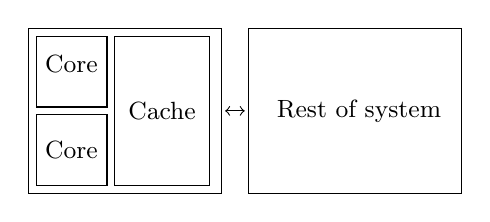
\begin{tikzpicture}
\draw (-0.5, -0.5) rectangle ++(0.9, 0.9);
\draw (-0.05, 0.05) node {\small Core};

\draw (-0.5, -1.5) rectangle ++(0.9, 0.9);
\draw (-0.05, -1.05) node {\small Core};

\draw (0.5, -1.5) rectangle ++(1.2, 1.9);
\draw (1.1, -.55) node {\small Cache};

\draw (-0.6, -1.6) rectangle ++(2.45, 2.1);

\draw (2.2, -1.6) rectangle ++(2.7, 2.1);
\draw (3.6, -0.55) node {\small Rest of system};

\draw[<->] (1.9, -0.55) -- (2.15, -0.55);
\end{tikzpicture}
\end{center}
\hfill (credit: \emph{Multicore Application Programming}, p. 5)

This above Symmetric Multithreading (SMP) design is especially good for the 1:1 threading model. In
this case, the design of the cores don't need to change much, but they
still need to communicate with each other and the rest of the system.

Or, we can have a design that works well for the N:1 model:
\begin{center}
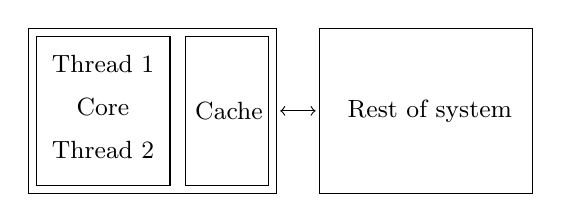
\begin{tikzpicture}
\draw (-1.4, -1.5) rectangle ++(1.7, 1.9);
\draw (-0.55, 0.05) node {\small Thread 1};
\draw (-0.55, -1.05) node {\small Thread 2};
\draw (-0.55, -0.5) node {\small Core};

\draw (0.5, -1.5) rectangle ++(1.05, 1.9);
\draw (1.05, -.55) node {\small Cache};

\draw (-1.5, -1.6) rectangle ++(3.15, 2.1);

\draw (2.2, -1.6) rectangle ++(2.7, 2.1);
\draw (3.6, -0.55) node {\small Rest of system};

\draw[<->] (1.7, -0.55) -- (2.15, -0.55);
\end{tikzpicture}
\end{center}

One would expect that executing two threads on one core might
mean that each thread would run more slowly. It depends on the instruction
mix. If the threads are trying to access the same resource, then each
thread would run more slowly. If they're doing different things, there's 
potential for speedup.

Finally, it's possible to both use multiple cores and put multiple threads
onto one core, as in the M:N model:

\begin{center}
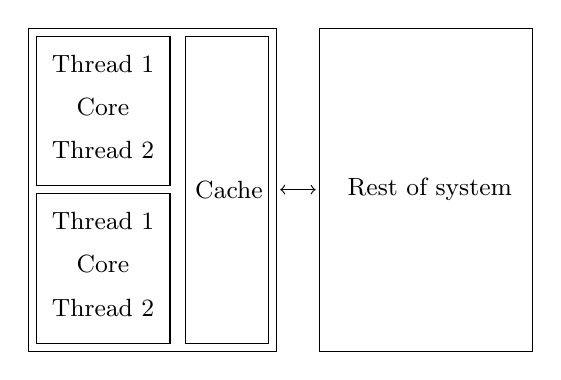
\begin{tikzpicture}

 \draw (-1.4, -1.5) rectangle +(1.7, 1.9);
 \draw (-1.4, -3.5) rectangle +(1.7, 1.9);

\foreach \y in {-2, 0}
{
 \draw (-0.55, 0.05) + (0, \y) node {\small Thread 1};
 \draw (-0.55, -1.05) + (0, \y) node {\small Thread 2};
 \draw (-0.55, -0.5) + (0, \y) node {\small Core};
}

\draw (0.5, -3.5) rectangle ++(1.05, 3.9);
\draw (1.05, -1.55) node {\small Cache};

\draw (-1.5, -3.6) rectangle ++(3.15, 4.1);

\draw (2.2, -3.6) rectangle ++(2.7, 4.1);
\draw (3.6, -1.55) node {\small Rest of system};

\draw[<->] (1.7, -1.55) -- (2.15, -1.55);
\end{tikzpicture}
\end{center}
Here we have four hardware threads; pairs of threads share hardware
resources. One example of a processor which supports chip multi-threading
(CMT) is the UltraSPARC T2, which has 8 cores, each of which supports 8 
threads. All of the cores share a common level 2 cache.

\paragraph{Non-SMP systems.} The designs we've seen above have been
more or less SMP designs; all of the cores are mostly alike.
A very non-Smp system is the Cell, which contains a PowerPC main core
(the PPE) and 7 Synergistic Processing Elements (SPEs), which are
small vector computers.


\paragraph{Non-Uniform Memory Access.}
In SMP systems, all CPUs have approximately the same access time for resources
(subject to cache misses). There are also NUMA, or Non-Uniform Memory Access,
systems out there. In that case, CPUs can access different resources at different
speeds. (Resources goes beyond just memory).

In this case, the operating system should schedule tasks on CPUs which
can access resources faster.  Since memory is commonly the bottleneck,
each CPU has its own memory bank.

\paragraph{Using CMT effectively.} Typically, a CPU will expose its
hardware threads using virtual CPUs.
In current hardware designs, each of the hardware threads has the same
performance. 

However, performance varies depending on context. In the above
example, two threads running on the same core will most probably run
more slowly than two threads running on separate cores, since they'd
contend for the same core's resources. Task switches between cores (or
CPUs!) are also slow, as they may involve reloading caches.

Solaris ``processor sets''
enable that operating system to assign processes to specific virtual CPUs,
while Linux's ``affinity'' keeps a process running on the same virtual CPU.
Both of these features reduce the number of task switches, and processor
sets can help reduce resource contention, along with Solaris's locality
groups\footnote{Gove suggests that locality groups help reduce contention
for core resources, but they seem to help more with memory.}

\section*{Processes versus Threads}
The first design decision that you need to solve when parallelizing programs
is whether you should use threads or processes.

  \begin{itemize}
    \item Threads are basically light-weight processes which piggy-back on
          processes' address space.
  \end{itemize}

Traditionally (pre-Linux 2.6) you had to use {\tt
  fork}~(for~processes) and {\tt clone} (for threads). But {\tt clone}
is not POSIX compliant, and its man page says that it's
Linux-specific---FreeBSD uses {\tt rfork()}. (POSIX is the standard
for Unix-like operating systems).

\paragraph{When processes are better.} {\tt fork} is safer and more secure than threads.

  \begin{enumerate}
    \item Each process has its own virtual address space:
      \begin{itemize}
        \item Memory pages are not copied, they are copy-on-write. Therefore, processes use less memory than you would expect.
      \end{itemize}
    \item Buffer overruns or other security holes do not expose other~processes.
    \item If a process crashes, the others can continue.
  \end{enumerate}

{\bf Example:} In the Chrome browser, each tab is a separate
process. Scott McCloud explained this:
\url{http://uncivilsociety.org/2008/09/google-chrome-comic-by-scott-m.html}.

\paragraph{When threads are better.} Threads are easier and faster.

  \begin{enumerate}
    \item Interprocess communication (IPC) is more complicated and slower than interthread
          communication; must use operating system utilities (pipes, semaphores, shared
              memory, etc) instead of thread library (or just memory reads and writes).
    \item Processes have much higher startup, shutdown and synchronization costs than threads.
    \item Pthreads fix the issues of {\tt clone} and provide a
          uniform interface for most systems. (You'll work with them in Assignment 1.)
  \end{enumerate}

\paragraph{How to choose?}
  If your application is like this:
  \begin{itemize}
    \item mostly independent tasks, with little or no communication;
    \item task startup and shutdown costs are negligible compared to overall runtime; and
    \item want to be safer against bugs and security holes,
  \end{itemize}
then processes are the way to go. If it's the opposite of this, then use threads.

 For performance reasons, along with ease and consistency across systems, we'll use threads, and Pthreads in particular.


\end{document}
